\documentclass[10pt,aspectratio=169]{beamer}

%================================================
% Theme
%================================================
\usetheme[numbering=fraction,progressbar=frametitle]{metropolis}

%================================================
% Packages
%================================================
\usepackage{amsmath,amssymb}
\usepackage{booktabs}
\usepackage{array}
\usepackage{tikz}
\usetikzlibrary{automata,positioning,arrows.meta,calc}
\usepackage[useregional]{datetime2}
\usepackage{xcolor}
\usepackage{listings}

%================================================
% Metadata
%================================================
\newcommand{\LastCompiled}{\DTMnow}

\title{Theory of Computation}
\subtitle{Lecture 4: Deterministic Finite Automata}
\author{Sheikh Azizul Hakim\\Lecturer, Department of CSE, BUET}
\date{Last compiled: \LastCompiled}

%================================================
% Convenience Macros
%================================================
\newcommand{\eps}{\varepsilon}
\newcommand{\blank}{\sqcup}
\newcommand{\Yes}{\textsc{Yes}}
\newcommand{\No}{\textsc{No}}
\newcommand{\lang}[1]{\mathsf{#1}}
\newcommand{\dfa}{M=(Q,\Sigma,\delta,q_0,F)}

\tikzset{
  dfastate/.style={state,minimum size=8mm,inner sep=1pt},
  smallstate/.style={state,minimum size=7mm,inner sep=1pt},
  every edge/.style={draw,->,>=Stealth,shorten >=1pt},
}

%================================================
% Listings
%================================================
\lstdefinestyle{code}{
  basicstyle=\ttfamily\small,
  frame=single,
  backgroundcolor=\color{black!4},
  rulecolor=\color{black!20},
  showstringspaces=false,
  columns=fullflexible,
  keepspaces=true
}
\lstset{style=code}

%================================================
\begin{document}

%================================================
\maketitle

%================================================
\begin{frame}[standout]
How do we describe finite memory precisely?
\end{frame}

%================================================
\section{4A. From State Diagrams to Mathematical Models}

%================================================
\begin{frame}{Where We Are in the Story}

\begin{center}
\begin{tabular}{lll}
\toprule
\textbf{Lecture} & \textbf{Question} & \textbf{Main idea}\\
\midrule
1 & Why study computation? & Limits of machines\\
2 & What are problems? & Languages as sets of strings\\
3 & What can finite memory do? & State machines\\
4 & How do we specify them? & Deterministic finite automata\\
\bottomrule
\end{tabular}
\end{center}

\vspace{1em}

Today we turn intuition into a precise mathematical object.

\end{frame}

%================================================
\begin{frame}{Communicating a Machine}

Suppose you designed a password validator or a tokenizer.

\vspace{1em}

How can you communicate the design to someone else?

\pause

\begin{itemize}
\item A drawing can be intuitive.
\pause
\item A mathematical specification is precise.
\pause
\item A table can define one part of the mathematics.
\end{itemize}

\vspace{1em}

In theory, we need descriptions that are clear, compact, and unambiguous.

\end{frame}

%================================================
\begin{frame}{Two Views of the Same Machine}

\begin{center}
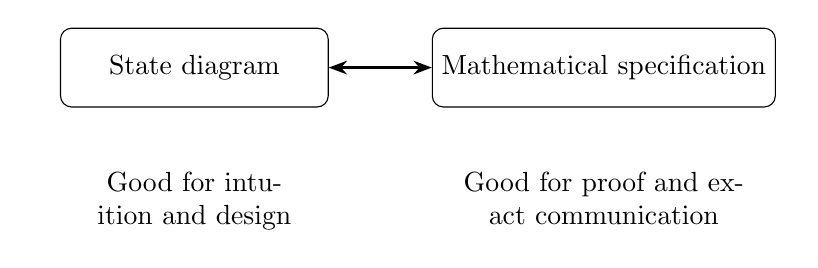
\begin{tikzpicture}[node distance=5.2cm]

\node[draw,rounded corners,minimum width=3.4cm,minimum height=1cm] (g)
{State diagram};

\node[draw,rounded corners,minimum width=4.2cm,minimum height=1cm,right of=g] (m)
{Mathematical specification};

\draw[<->,>=Stealth,thick] (g) -- (m);

\node[below=0.7cm of g,text width=4cm,align=center]
{Good for intuition and design};

\node[below=0.7cm of m,text width=4.5cm,align=center]
{Good for proof and exact communication};

\end{tikzpicture}
\end{center}

\vspace{1em}

A transition table is simply one convenient way to define the transition function.

\end{frame}

%================================================
\begin{frame}{Why Mathematicians Love Tuples}

A point is described by two coordinates:
\[
(3,5).
\]

\pause

A graph is described by vertices and edges:
\[
G=(V,E).
\]

\pause

A student record may be described by several fields:
\[
(\text{Name},\text{ID},\text{CGPA}).
\]

\pause

Whenever an object has several components, mathematics often packages them into a tuple.

\end{frame}

%================================================
\begin{frame}{A DFA Has Five Ingredients}

To describe a deterministic finite automaton, we need:

\pause

\begin{enumerate}
\item a finite set of states,
\pause
\item an input alphabet,
\pause
\item a rule for moving between states,
\pause
\item a start state,
\pause
\item a set of accepting states.
\end{enumerate}

\pause

So we write
\[
\dfa.
\]

\end{frame}

%================================================
\begin{frame}{Definition: Deterministic Finite Automaton}

A \textbf{deterministic finite automaton}, or DFA, is a 5-tuple
\[
M=(Q,\Sigma,\delta,q_0,F),
\]
where

\begin{itemize}
\item $Q$ is a finite set of states,
\item $\Sigma$ is a finite input alphabet,
\item $\delta:Q\times\Sigma\rightarrow Q$ is the transition function,
\item $q_0\in Q$ is the start state,
\item $F\subseteq Q$ is the set of accepting states.
\end{itemize}

\end{frame}

%================================================
\begin{frame}{The Running Example: Even Number of 1's}

Language we want to recognize:
\[
\lang{EVEN}_1=\{w\in\{0,1\}^*: w\text{ contains an even number of }1\text{'s}\}.
\]

\pause

What information must the machine remember?

\pause

Only whether the number of $1$'s seen so far is even or odd.

\[
q_E: \text{even number of }1\text{'s seen},
\qquad
q_O: \text{odd number of }1\text{'s seen}.
\]

\end{frame}

%================================================
\begin{frame}{The Same Machine as a Diagram}

\begin{center}
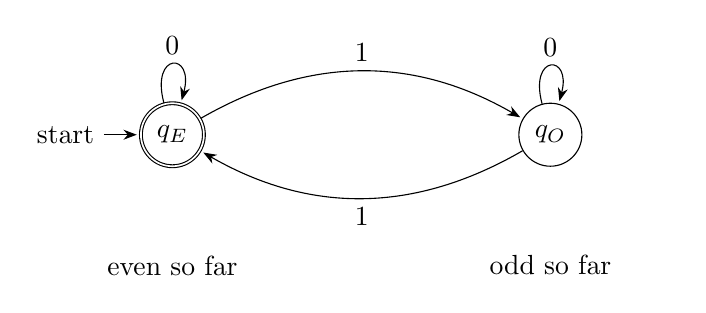
\begin{tikzpicture}[->,>=Stealth,shorten >=1pt,node distance=4.8cm]

\node[dfastate,initial,accepting] (e) {$q_E$};
\node[dfastate,right of=e] (o) {$q_O$};

\path
(e) edge[loop above] node {$0$} ()
(e) edge[bend left] node[above] {$1$} (o)
(o) edge[loop above] node {$0$} ()
(o) edge[bend left] node[below] {$1$} (e);

\node[below=1.0cm of e,text width=3cm,align=center] {even so far};
\node[below=1.0cm of o,text width=3cm,align=center] {odd so far};

\end{tikzpicture}
\end{center}

\vspace{0.5em}

States are not merely circles; they encode the information remembered by the machine.

\end{frame}

%================================================
\begin{frame}{The Same Machine as Mathematics}

\[
Q=\{q_E,q_O\},
\qquad
\Sigma=\{0,1\},
\qquad
q_0=q_E,
\qquad
F=\{q_E\}.
\]

\pause

The transition function $\delta$ is defined by
\[
\begin{array}{c|cc}
\delta & 0 & 1\\
\hline
q_E & q_E & q_O\\
q_O & q_O & q_E
\end{array}
\]

\pause

This table is not a third representation; it is simply a compact definition of $\delta$.

\end{frame}

%================================================
\begin{frame}{What Does $\delta:Q\times\Sigma\to Q$ Mean?}

The transition function consumes two pieces of information:
\[
(\text{current state},\text{next input symbol}).
\]

\pause

It returns one piece of information:
\[
\text{new state}.
\]

\pause

For example,
\[
\delta(q_E,1)=q_O,
\qquad
\delta(q_O,0)=q_O.
\]

\pause

This is the mathematical version of ``follow the arrow labeled by the symbol.''

\end{frame}

%================================================
\begin{frame}{Why Is It Called Deterministic?}

For every pair
\[
(q,a)\in Q\times\Sigma,
\]
there is exactly one next state
\[
\delta(q,a)\in Q.
\]

\vspace{1em}

\pause

No guessing.

No ambiguity.

No missing transition.

Exactly one next state.

\end{frame}

%================================================
\begin{frame}{What Does a State Remember?}

For the parity machine, the state does not remember the whole input.

\pause

After reading
\[
101001101001101,
\]
we do not remember every symbol.

\pause

We remember only one fact:
\[
\text{the parity of the number of }1\text{'s seen so far}.
\]

\pause

This is the central design idea of finite automata:
\[
\text{compress the relevant past into finitely many states.}
\]

\end{frame}

%================================================
\begin{frame}[standout]
A DFA is finite memory plus a deterministic update rule.
\end{frame}

%================================================
\section{4B. Acceptance, Rejection, and Languages}

%================================================
\begin{frame}{Running a DFA on an Input}

Input:
\[
1100101.
\]

\pause

Computation:
\[
q_E
\xrightarrow{1}
q_O
\xrightarrow{1}
q_E
\xrightarrow{0}
q_E
\xrightarrow{0}
q_E
\xrightarrow{1}
q_O
\xrightarrow{0}
q_O
\xrightarrow{1}
q_E.
\]

\pause

The final state is $q_E$, and $q_E\in F$.

Therefore the input is accepted.

\end{frame}

%================================================
\begin{frame}{Formal Acceptance Without New Notation}

Let
\[
M=(Q,\Sigma,\delta,q_0,F)
\]
be a DFA, and let
\[
w=w_1w_2\cdots w_n
\]
be an input string over $\Sigma$.

\pause

The machine accepts $w$ if there is a sequence of states
\[
r_0,r_1,\ldots,r_n
\]
such that

\begin{enumerate}
\item $r_0=q_0$,
\item $\delta(r_i,w_{i+1})=r_{i+1}$ for $0\le i\le n-1$,
\item $r_n\in F$.
\end{enumerate}

\end{frame}

%================================================
\begin{frame}{What About the Empty String?}

The empty string is
\[
\eps.
\]

It has length zero.

\pause

If the input is $\eps$, the DFA reads no symbols.

\pause

So it remains in the start state $q_0$.

\pause

Therefore:

\begin{center}
A DFA accepts $\eps$ exactly when $q_0\in F$.
\end{center}

\end{frame}

%================================================
\begin{frame}{The Language of a DFA}

A DFA may accept some strings and rejects others.

\pause

The language of $M$ is the set of all strings accepted by $M$:
\[
L(M)=\{w\in\Sigma^*: M\text{ accepts }w\}.
\]

\pause

This connects back to Lecture 2:

\begin{center}
Machines recognize languages.
\end{center}

\end{frame}

%================================================
\begin{frame}{Three Similar-Looking Objects}

These are different:

\vspace{0.5em}

\begin{center}
\begin{tabular}{lll}
\toprule
\textbf{Notation} & \textbf{Meaning} & \textbf{Size}\\
\midrule
$\eps$ & the empty string & length $0$\\
$\emptyset$ & the empty language & $0$ strings\\
$\{\eps\}$ & language containing only the empty string & $1$ string\\
\bottomrule
\end{tabular}
\end{center}

\pause

\vspace{1em}

Common mistake:
\[
\emptyset \ne \{\eps\}.
\]

\end{frame}

%================================================
\begin{frame}{A DFA for the Empty Language}

Language:
\[
L=\emptyset.
\]

\begin{center}
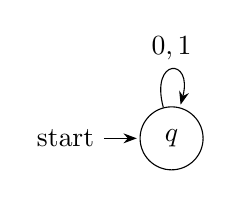
\begin{tikzpicture}[->,>=Stealth,shorten >=1pt,node distance=3cm]
\node[dfastate,initial] (q) {$q$};
\path (q) edge[loop above] node {$0,1$} ();
\end{tikzpicture}
\end{center}

\pause

Specification over $\Sigma=\{0,1\}$:
\[
Q=\{q\},\qquad q_0=q,\qquad F=\emptyset.
\]

No state is accepting, so no string is accepted.

\end{frame}

%================================================
\begin{frame}{A DFA for the Language $\{\eps\}$}

Language:
\[
L=\{\eps\}.
\]

\begin{center}
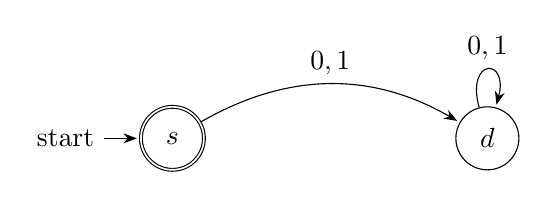
\begin{tikzpicture}[->,>=Stealth,shorten >=1pt,node distance=4cm]
\node[dfastate,initial,accepting] (s) {$s$};
\node[dfastate,right of=s] (d) {$d$};
\path
(s) edge[bend left] node[above] {$0,1$} (d)
(d) edge[loop above] node {$0,1$} ();
\end{tikzpicture}
\end{center}

\pause

The start state is accepting, so $\eps$ is accepted.

Any nonempty input moves to the dead state $d$.

\end{frame}

%================================================
\begin{frame}{A DFA for $\Sigma^*$}

Language:
\[
L=\Sigma^*.
\]

\begin{center}
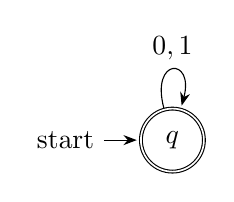
\begin{tikzpicture}[->,>=Stealth,shorten >=1pt,node distance=3cm]
\node[dfastate,initial,accepting] (q) {$q$};
\path (q) edge[loop above] node {$0,1$} ();
\end{tikzpicture}
\end{center}

\pause

Every string is accepted, including $\eps$.

\vspace{1em}

Notice the contrast:
\[
\emptyset,
\qquad
\{\eps\},
\qquad
\Sigma^*.
\]

\end{frame}

%================================================
\begin{frame}{Dead States}

A dead state represents a situation from which success is impossible.

\pause

Once the machine enters a dead state, it stays there forever.

\begin{center}
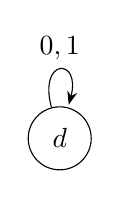
\begin{tikzpicture}[->,>=Stealth,shorten >=1pt,node distance=3cm]
\node[dfastate] (d) {$d$};
\path (d) edge[loop above] node {$0,1$} ();
\end{tikzpicture}
\end{center}

\pause

Dead states often make deterministic automata complete.

\end{frame}

%================================================
\begin{frame}{A Useful Analogy}

For a graph, we may specify edges using:

\begin{itemize}
\item a picture,
\item an adjacency list,
\item an adjacency matrix.
\end{itemize}

\pause

For a DFA, we may specify transitions using:

\begin{itemize}
\item a state diagram,
\item equations such as $\delta(q,0)=r$,
\item a transition table.
\end{itemize}

\pause

The object is the same; only the description changes.

\end{frame}

%================================================
\begin{frame}[standout]
A DFA recognizes a language: the set of all strings it accepts.
\end{frame}

%================================================
\section{4C. Worked Examples: Designing States}

%================================================
\begin{frame}{How to Design a DFA}

A good design strategy:

\begin{enumerate}
\item Decide what information must be remembered.
\item Make one state for each possible memory situation.
\item Define how each input symbol updates that information.
\item Mark the accepting states.
\end{enumerate}

\pause

The hardest step is almost always the first one.

\begin{center}
What information is enough?
\end{center}

\end{frame}

%================================================
\begin{frame}{Example 1: Strings Ending with 01}

Language:
\[
L=\{w\in\{0,1\}^*: w\text{ ends with }01\}.
\]

\pause

What should the states remember?

\begin{itemize}
\item Have we just seen a $0$?
\item Have we just seen $01$ at the end?
\end{itemize}

\pause

We do not need to remember the whole string.

\end{frame}

%================================================
\begin{frame}{DFA for Strings Ending with 01}

\begin{center}
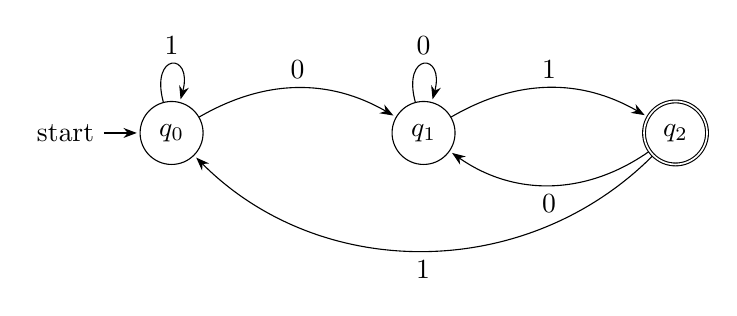
\begin{tikzpicture}[->,>=Stealth,shorten >=1pt,node distance=3.2cm]

\node[dfastate,initial] (q0) {$q_0$};
\node[dfastate,right of=q0] (q1) {$q_1$};
\node[dfastate,accepting,right of=q1] (q2) {$q_2$};

\path
(q0) edge[loop above] node {$1$} ()
(q0) edge[bend left] node[above] {$0$} (q1)
(q1) edge[loop above] node {$0$} ()
(q1) edge[bend left] node[above] {$1$} (q2)
(q2) edge[bend left=35] node[below] {$0$} (q1)
(q2) edge[bend left=45] node[below] {$1$} (q0);

\end{tikzpicture}
\end{center}

\vspace{0.5em}

$q_2$ means: the input read so far ends with $01$.

\end{frame}

%================================================
\begin{frame}{Specification for Strings Ending with 01}

\[
Q=\{q_0,q_1,q_2\},
\qquad
\Sigma=\{0,1\},
\qquad
F=\{q_2\}.
\]

\[
\begin{array}{c|cc}
\delta & 0 & 1\\
\hline
q_0 & q_1 & q_0\\
q_1 & q_1 & q_2\\
q_2 & q_1 & q_0
\end{array}
\]

\pause

The table is a compact definition of the arrows in the diagram.

\end{frame}

%================================================
\begin{frame}{Trace: Does 1101 End with 01?}

Input:
\[
1101.
\]

\pause

Computation:
\[
q_0
\xrightarrow{1}
q_0
\xrightarrow{1}
q_0
\xrightarrow{0}
q_1
\xrightarrow{1}
q_2.
\]

\pause

Since $q_2\in F$, the input is accepted.

\end{frame}

%================================================
\begin{frame}{Example 2: Strings Containing 001}

Language:
\[
L=\{w\in\{0,1\}^*: w\text{ contains }001\text{ as a substring}\}.
\]

\pause

What should the states remember?

\pause

The longest suffix of the input so far that is also a prefix of $001$.

\begin{itemize}
\item nothing useful yet,
\item just saw $0$,
\item just saw $00$,
\item have seen $001$.
\end{itemize}

\end{frame}

%================================================
\begin{frame}{DFA for Strings Containing 001}

\begin{center}
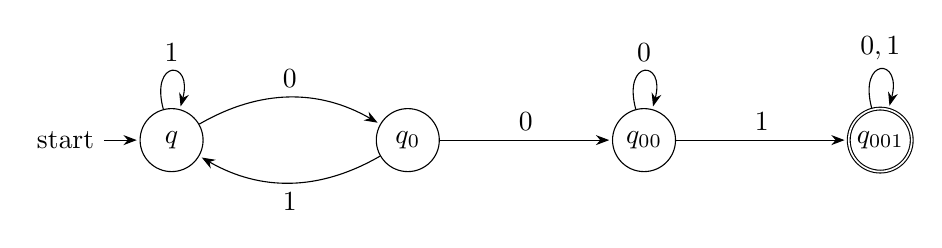
\begin{tikzpicture}[->,>=Stealth,shorten >=1pt,node distance=3.0cm]

\node[dfastate,initial] (q0) {$q$};
\node[dfastate,right of=q0] (q1) {$q_0$};
\node[dfastate,right of=q1] (q2) {$q_{00}$};
\node[dfastate,accepting,right of=q2] (q3) {$q_{001}$};

\path
(q0) edge[loop above] node {$1$} ()
(q0) edge[bend left] node[above] {$0$} (q1)
(q1) edge[bend left] node[below] {$1$} (q0)
(q1) edge node[above] {$0$} (q2)
(q2) edge[loop above] node {$0$} ()
(q2) edge node[above] {$1$} (q3)
(q3) edge[loop above] node {$0,1$} ();

\end{tikzpicture}
\end{center}

\vspace{0.5em}

Once $001$ appears, the machine stays accepting forever.

\end{frame}

%================================================
\begin{frame}{Why the Loop on $q_{00}$ with 0?}

Suppose we have seen
\[
000.
\]

\pause

The last two symbols are still
\[
00.
\]

\pause

So after reading another $0$ from state $q_{00}$, we remain in $q_{00}$.

\vspace{1em}

This is a common pattern in substring-matching automata.

\end{frame}

%================================================
\begin{frame}{Example 3: No Three Consecutive b's}

Language:
\[
L=\{w\in\{a,b\}^*: w\text{ does not contain }bbb\text{ as a substring}\}.
\]

\pause

What should the states remember?

\pause

Only the number of consecutive $b$'s at the end:
\[
0,\qquad 1,
\qquad 2,
\qquad \text{too many}.
\]

\end{frame}

%================================================
\begin{frame}{DFA for No Three Consecutive b's}

\begin{center}
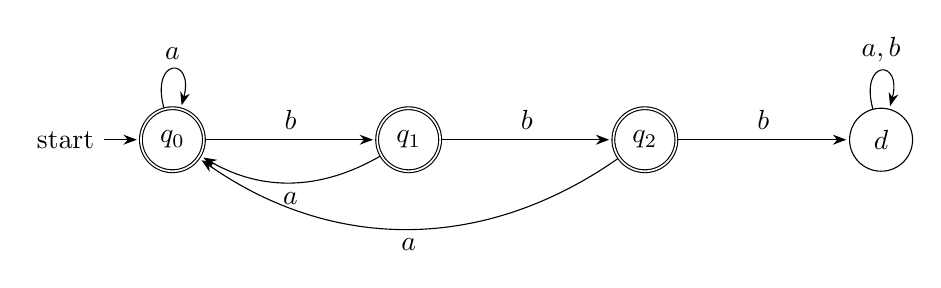
\begin{tikzpicture}[->,>=Stealth,shorten >=1pt,node distance=3.0cm]

\node[dfastate,initial,accepting] (q0) {$q_0$};
\node[dfastate,accepting,right of=q0] (q1) {$q_1$};
\node[dfastate,accepting,right of=q1] (q2) {$q_2$};
\node[dfastate,right of=q2] (d) {$d$};

\path
(q0) edge[loop above] node {$a$} ()
(q0) edge node[above] {$b$} (q1)
(q1) edge[bend left] node[below] {$a$} (q0)
(q1) edge node[above] {$b$} (q2)
(q2) edge[bend left=35] node[below] {$a$} (q0)
(q2) edge node[above] {$b$} (d)
(d) edge[loop above] node {$a,b$} ();

\end{tikzpicture}
\end{center}

\vspace{0.5em}

Here $d$ is a dead state: once $bbb$ appears, success is impossible.

\end{frame}

%================================================
\begin{frame}{Lesson from the First Three Examples}

The state should remember exactly what is relevant:

\begin{center}
\begin{tabular}{ll}
\toprule
\textbf{Language} & \textbf{Information remembered}\\
\midrule
Even number of $1$'s & parity\\
Ends with $01$ & relevant suffix\\
Contains $001$ & progress toward pattern\\
No $bbb$ & recent run of $b$'s\\
\bottomrule
\end{tabular}
\end{center}

\pause

Good automaton design is information design.

\end{frame}

%================================================
\section{4D. Worked Examples: Beyond the Obvious}

%================================================
\begin{frame}{Example 4: Binary Numbers Divisible by 3}

Language:
\[
L=\{w\in\{0,1\}^*: w\text{ is the binary representation of a number divisible by }3\}.
\]

\pause

At first this looks arithmetic, not automata.

\pause

But we only need to remember the remainder modulo $3$.

\[
q_0: \text{remainder }0,
\qquad
q_1: \text{remainder }1,
\qquad
q_2: \text{remainder }2.
\]

\end{frame}

%================================================
\begin{frame}{Updating Remainders}

If the current value has remainder $r$ modulo $3$, and we append bit $b$, the new value is
\[
2r+b \pmod 3.
\]

\pause

Why?

Appending a bit to the right doubles the old binary number and adds the new bit.

\pause

So the transition rule is
\[
r\mapsto 2r+b \pmod 3.
\]

\end{frame}

%================================================
\begin{frame}{DFA for Divisibility by 3}

\begin{center}
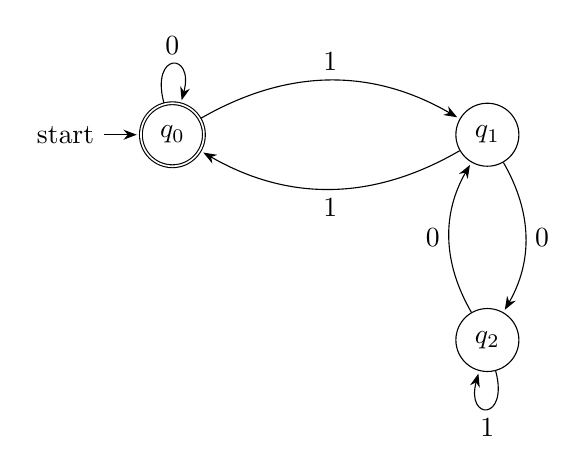
\begin{tikzpicture}[->,>=Stealth,shorten >=1pt,node distance=4.0cm]

\node[dfastate,initial,accepting] (q0) {$q_0$};
\node[dfastate,right of=q0] (q1) {$q_1$};
\node[dfastate,below=2.2cm of $(q1)$] (q2) {$q_2$};

\path
(q0) edge[loop above] node {$0$} ()
(q0) edge[bend left] node[above] {$1$} (q1)
(q1) edge[bend left] node[below] {$1$} (q0)
(q1) edge[bend left] node[right] {$0$} (q2)
(q2) edge[bend left] node[left] {$0$} (q1)
(q2) edge[loop below] node {$1$} ();

\end{tikzpicture}
\end{center}

\vspace{0.5em}

Accept when the remainder is $0$.

\end{frame}

%================================================
\begin{frame}{Trace: Is 110 Divisible by 3?}

Binary string:
\[
110_2=6.
\]

\pause

Computation:
\[
q_0
\xrightarrow{1}
q_1
\xrightarrow{1}
q_0
\xrightarrow{0}
q_0.
\]

\pause

Final state $q_0$ is accepting.

Therefore $110_2$ is accepted.

\end{frame}

%================================================
\begin{frame}{Example 5: Exactly the String 1011}

Language:
\[
L=\{1011\}.
\]

\pause

What should the machine remember?

\pause

How much of the target string has been matched so far.

\[
\text{matched nothing},
\quad 1,
\quad 10,
\quad 101,
\quad 1011.
\]

\pause

Any wrong move goes to a dead state.

\end{frame}

%================================================
\begin{frame}{DFA for Exactly 1011}

\begin{center}
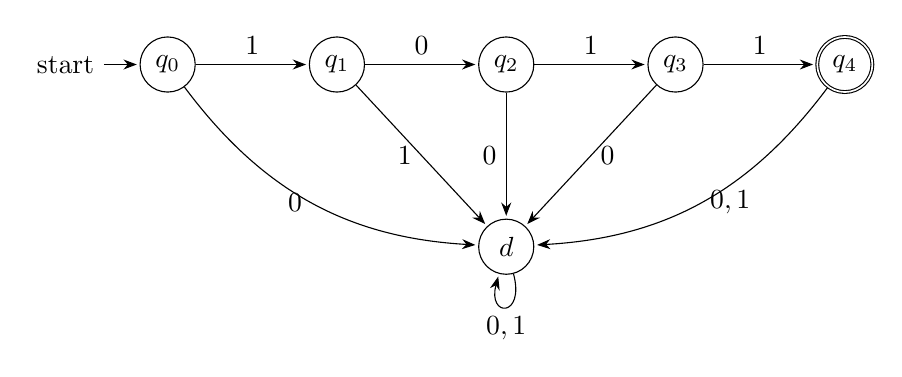
\begin{tikzpicture}[->,>=Stealth,shorten >=1pt,node distance=2.15cm]

\node[smallstate,initial] (q0) {$q_0$};
\node[smallstate,right of=q0] (q1) {$q_1$};
\node[smallstate,right of=q1] (q2) {$q_2$};
\node[smallstate,right of=q2] (q3) {$q_3$};
\node[smallstate,accepting,right of=q3] (q4) {$q_4$};
\node[smallstate,below=1.6cm of q2] (d) {$d$};

\path
(q0) edge node[above] {$1$} (q1)
(q1) edge node[above] {$0$} (q2)
(q2) edge node[above] {$1$} (q3)
(q3) edge node[above] {$1$} (q4)
(q0) edge[bend right=25] node[left] {$0$} (d)
(q1) edge node[left] {$1$} (d)
(q2) edge node[left] {$0$} (d)
(q3) edge node[right] {$0$} (d)
(q4) edge[bend left=25] node[right] {$0,1$} (d)
(d) edge[loop below] node {$0,1$} ();

\end{tikzpicture}
\end{center}

\vspace{0.5em}

The accepting state is reached only after reading exactly $1011$.

\end{frame}

%================================================
\begin{frame}{Example 6: A Fixed Keyword}

Language:
\[
L=\{\texttt{if}\}.
\]

\pause

This is the tiny version of what lexical analyzers do.

\pause

To recognize a fixed keyword, the states remember how much of the keyword has been matched.

\[
\texttt{Start}
\rightarrow \texttt{i}\rightarrow \texttt{if}.
\]

\pause

Real tokenizers combine many such patterns.

\end{frame}

%================================================
\begin{frame}{Example 7: Password Rule}

Suppose passwords are over
\[
\Sigma=\{a,b,0,1\}
\]
and must contain at least one digit.

\pause

What should the states remember?

\pause

Only whether a digit has already appeared.

\[
q_N: \text{no digit yet},
\qquad
q_D: \text{digit has appeared}.
\]

\pause

This is finite memory.

\end{frame}

%================================================
\begin{frame}{DFA for ``Contains a Digit''}

\begin{center}
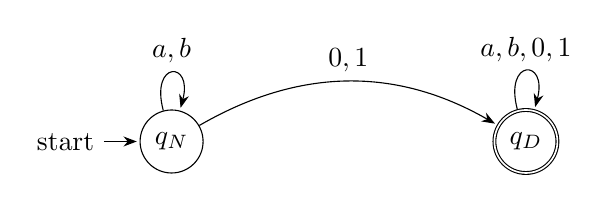
\begin{tikzpicture}[->,>=Stealth,shorten >=1pt,node distance=4.5cm]

\node[dfastate,initial] (n) {$q_N$};
\node[dfastate,accepting,right of=n] (d) {$q_D$};

\path
(n) edge[loop above] node {$a,b$} ()
(n) edge[bend left] node[above] {$0,1$} (d)
(d) edge[loop above] node {$a,b,0,1$} ();

\end{tikzpicture}
\end{center}

\pause

The machine does not remember the password.

It remembers only whether the rule has already been satisfied.

\end{frame}

%================================================
\begin{frame}{Conceptual Boundary}

These fit naturally into finite-state machines:

\begin{itemize}
\item fixed keywords,
\item fixed suffixes,
\item fixed substrings,
\item parity,
\item remainders modulo a fixed number,
\item fixed password rules.
\end{itemize}

\pause

They require only finitely many memory situations.

\end{frame}

%================================================
\begin{frame}{Prediction Game}

Which of these should be recognizable by a DFA?

\begin{enumerate}
\item Strings with an even number of $1$'s.
\item Strings ending with $001$.
\item Strings containing $001$.
\item Strings with equal numbers of $0$'s and $1$'s.
\item Balanced parentheses.
\item Valid JSON strings.
\end{enumerate}

\pause

The first three are regular.

The last three need more memory.

\end{frame}

%================================================
\begin{frame}{Why Equal Counts Feel Different}

Consider
\[
0^n1^n.
\]

To check whether the number of $0$'s equals the number of $1$'s, the machine seems to need to remember an unbounded count.

\pause

A DFA has only finitely many states.

\pause

This tension will lead us to nonregular languages and the pumping lemma.

\end{frame}

%================================================
\begin{frame}{Why Balanced Parentheses Feel Different}

To recognize
\[
(),\quad (()),\quad ((()())),\quad \ldots
\]

we need to remember how many open parentheses are currently unmatched.

\pause

That number can grow without bound.

\pause

This will motivate pushdown automata and context-free languages later.

\end{frame}

%================================================
\begin{frame}{What You Should Be Able to Do Now}

Given a DFA, you should be able to:

\begin{itemize}
\item identify $Q,\Sigma,\delta,q_0,F$,
\item explain what each state remembers,
\item trace an input string,
\item decide whether the string is accepted,
\item describe the language recognized by the DFA.
\end{itemize}

\pause

Given a simple language, you should begin by asking:

\begin{center}
What finite information is enough?
\end{center}

\end{frame}

%================================================
\begin{frame}{Suggested Exercises}

Design DFAs for the following languages over $\{0,1\}$:

\begin{enumerate}
\item strings ending with $00$,
\item strings containing at least one $1$,
\item strings containing exactly one $1$,
\item strings whose length is divisible by $3$,
\item strings that do not contain $11$,
\item the language $\emptyset$,
\item the language $\{\eps\}$.
\end{enumerate}

\end{frame}

%================================================
\begin{frame}[standout]
A DFA is not merely a diagram.

It is a mathematical object that recognizes a language using finite memory.
\end{frame}

%================================================
\end{document}
